\input{../../../.preambles/02-lab_work}
\input{../../../.preambles/30-physics}
\newgeometry{top=1.5cm, bottom=1.5cm, left=1cm, right=1cm}
\newcommand{\el}[3]{\nucleus{#3}{#2}{#1}}
\begin{document}
    \begin{table}[h!]
        \center
        \begin{tabular}{|C{.5}|C{.2}|C{.25}|}
            \hline
            \multicolumn{1}{|c|}{\multirow{4}{*}{Лабораторная работа № 5}} &
            Студент, группа & {{ student }}, Ф-369 \\ \cline{2-3}
            & Дата выполнения & 06.03.2013 \\ \cline{2-3}
            & Подпись &  \\ \cline{2-3}
            Энергетические соотношения для бета-распада & Дата отчёта & \\ \cline{2-3}
            & Оценка &  \\ \cline{2-3}
            & Подпись &  \\ \hline
        \end{tabular}
    \end{table}

    \emph{Цель работы:} Ознакомиться с энергетическими соотношениями для
    \( \beta \)-распада и на основе экспериментальных значений энергий связи
    построить семейства парабол, иллюстрирующих \( \beta \)-превращения для
    чётных и нечётных значений массового числа \( A \).
    
    \subsection{Чётные значения массового числа \emph{А}}
    
    \begin{table}[h!]
        \center
        \caption{\( A = 80 \)}
        \begin{tabular}{|C{.08}|C{.065}|C{.02}|C{.05}|C{.1}||C{.2}|C{.38}} \cline{1-6}
            Название & Элемент & \( Z \) & \( E_\emph{св} \), МэВ & Распад &
            Формула распада &
            \multirow{15}{*}{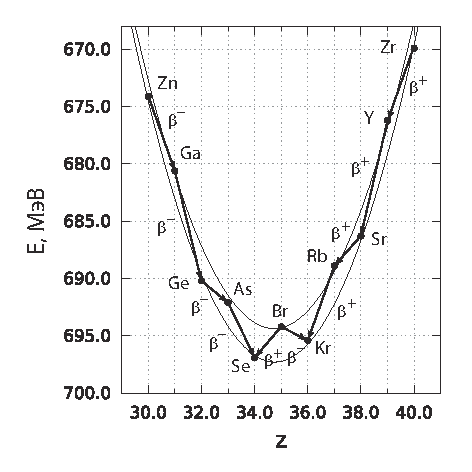
\includegraphics[width=.38\textwidth]{80}}
            \\ \cline{1-6}
            % -----------------------------------------
            Цинк & Zn & 30 & 674,1 & Бета\( ^- \) &
            \( \el{Zn}{80}{30}\, \to\ \el{Ga}{80}{31} + e^- + \tilde{\nu} \) &
            \\ \cline{1-5}
            Галлий & Ga & 31 & 680,6 & Бета\( ^- \) &
            \( \el{Ga}{80}{31}\, \to\ \el{Ge}{80}{32} + e^- + \tilde{\nu} \) &
            \\ \cline{1-5}
            Германий & Ge & 32 & 690,2 & Бета\( ^- \) &
            \( \el{Ge}{80}{32}\, \to\ \el{As}{80}{33} + e^- + \tilde{\nu} \) &
            \\ \cline{1-5}
            Мышьяк & As & 33 & 692,1 & Бета\( ^- \) &
            \( \el{As}{80}{33}\, \to\ \el{Se}{80}{34} + e^- + \tilde{\nu} \) &
            \\ \cline{1-5}
            Селен & Se & 34 & 696,9 & Стабильный изобар &
            \multirow{2}{*}{\( \el{Br}{80}{35}\, \to\ \el{Se}{80}{34} + e^+
            + \nu \)} & \\ \cline{1-5}
            Бром & Br & 35 & 694,2 & Бета\( ^+ \),~Бета\( ^- \) &
            \multirow{3}{*}{\( \el{Br}{80}{35} \to\ \el{Kr}{80}{36} + e^-
            + \tilde{\nu} \)} & \\ \cline{1-5}
            Криптон & Kr & 36 & 695,4 & Стабильный изобар & & \\ \cline{1-5}
            Рубидий & Rb & 37 & 688,9 & Бета\( ^+ \) &
            \( \el{Rb}{80}{37} \to\ \el{Kr}{80}{36} + e^+ + \nu \) &
            \\ \cline{1-5}
            Стронций & Sr & 38 & 686,3 & Бета\( ^+ \) &
            \( \el{Sr}{80}{38} \to\ \el{Rb}{80}{37} + e^+ + \nu \) &
            \\ \cline{1-5}
            Иттрий & Y & 39 & 676,2 & Бета\( ^+ \) &
            \( \el{Y}{80}{39} \to\ \el{Y}{80}{38} + e^+ + \nu \) &
            \\ \cline{1-5}
            Цирконий & Zr & 40 & 669,9 & Бета\( ^+ \) &
            \( \el{Zr}{80}{40} \to\ \el{Sr}{80}{39} + e^+ + \nu \) &
            \\ \cline{1-6}
        \end{tabular}
    \end{table}
    
    Энергия связи элемента \( \el{Se}{80}{34} \): \( E_\emph{св} = 697,\!6 \)~МэВ.

    Энергия связи элемента \( \el{Kr}{80}{36} \): \( E_\emph{св} = 698,\!3 \)~МэВ.

    \begin{table}[h!]
        \center
        \caption{\( A = 108 \)}
        \begin{tabular}{|C{.08}|C{.065}|C{.02}|C{.05}|C{.1}||C{.2}|C{.38}} \cline{1-6}
            Название & Элемент & \( Z \) & \( E_\emph{св} \), МэВ & Распад &
            Формула распада &
            \multirow{15}{*}{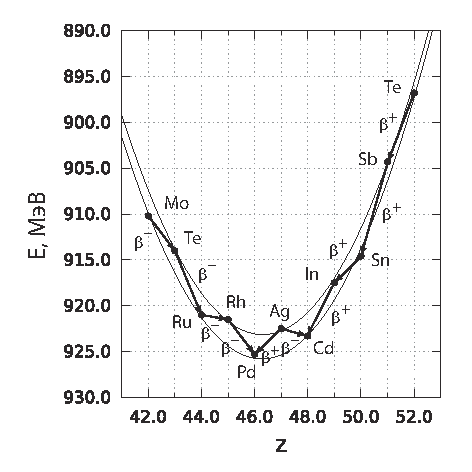
\includegraphics[width=.38\textwidth]{108}}
            \\ \cline{1-6}
            % -----------------------------------------
            Молибден & Mo & 42 & 910,2 & Бета\( ^- \) &
            \( \el{Mo}{108}{42}\, \to\ \el{Tc}{108}{43} + e^- + \tilde{\nu} \) &
            \\ \cline{1-5}
            Технеций & Tc & 43 & 914,0 & Бета\( ^- \) &
            \( \el{Tc}{108}{43}\, \to\ \el{Ru}{108}{44} + e^- + \tilde{\nu} \) &
            \\ \cline{1-5}
            Рутений & Ru & 44 & 921,0 & Бета\( ^- \) &
            \( \el{Ru}{108}{44}\, \to\ \el{Rh}{108}{45} + e^- + \tilde{\nu} \) &
            \\ \cline{1-5}
            Родий & Rh & 45 & 921,5 & Бета\( ^- \) &
            \( \el{Rh}{108}{45}\, \to\ \el{Pd}{108}{46} + e^- + \tilde{\nu} \) &
            \\ \cline{1-5}
            Палладий & Pd & 46 & 925,3 & Стабильный изобар &
            \multirow{2}{*}{\(\el{Ag}{108}{47}\, \to\ \el{Pd}{108}{46} + e^+
            + \nu \)} & \\ \cline{1-5}
            Серебро & Ag & 47 & 922,5 & Бета\( ^+ \),~Бета\( ^- \) &
            \multirow{3}{*}{\( \el{Ag}{108}{47} \to\ \el{Cd}{108}{48} + e^-
            + \tilde{\nu} \)} & \\ \cline{1-5}
            Кадмий & Cd & 48 & 923,4 & Стабильный изобар & & \\ \cline{1-5}
            Индий & In & 49 & 917,5 & Бета\( ^+ \) &
            \( \el{In}{108}{49} \to\ \el{Cd}{108}{48} + e^+ + \nu \) &
            \\ \cline{1-5}
            Олово & Sn & 50 & 914,6 & Бета\( ^+ \) &
            \( \el{Sn}{108}{50} \to\ \el{In}{108}{49} + e^+ + \nu \) &
            \\ \cline{1-5}
            Сурьма & Sb & 51 & 904,3 & Бета\( ^+ \) &
            \( \el{Sb}{108}{51} \to\ \el{Sn}{108}{50} + e^+ + \nu \) &
            \\ \cline{1-5}
            Теллур & Te & 52 & 896,8 & Бета\( ^+ \) &
            \( \el{Te}{108}{52} \to\ \el{Sb}{108}{51} + e^+ + \nu \) &
            \\ \cline{1-6}
        \end{tabular}
    \end{table}

    Энергия связи элемента \( \el{Pd}{108}{46} \): \( E_\emph{св} = 926,\!7 \)~МэВ.

    Энергия связи элемента \( \el{Cd}{108}{48} \): \( E_\emph{св} = 923,\!2 \)~МэВ.

    \pagebreak

    \begin{table}[h!]
        \center
        \caption{\( A = 128 \)}
        \begin{tabular}{|C{.08}|C{.065}|C{.02}|C{.05}|C{.1}||C{.2}|C{.38}} \cline{1-6}
            Название & Элемент & \( Z \) & \( E_\emph{св} \), МэВ & Распад &
            Формула распада &
            \multirow{15}{*}{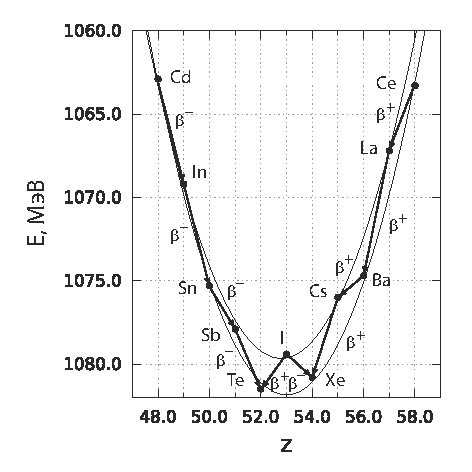
\includegraphics[width=.38\textwidth]{128}}
            \\ \cline{1-6}
            % -----------------------------------------
            Кадмий & Cd & 48 & 1062,9 & Бета\( ^- \) &
            \( \el{Cd}{128}{48}\, \to\ \el{In}{128}{49} + e^- + \tilde{\nu} \) &
            \\ \cline{1-5}
            Индий & In & 49 & 1069,2 & Бета\( ^- \) &
            \( \el{In}{128}{49}\, \to\ \el{Sn}{128}{50} + e^- + \tilde{\nu} \) &
            \\ \cline{1-5}
            Олово & Sn & 50 & 1075,3 & Бета\( ^- \) &
            \( \el{Sn}{128}{50}\, \to\ \el{Sb}{128}{51} + e^- + \tilde{\nu} \) &
            \\ \cline{1-5}
            Сурьма & Sb & 51 & 1077,9 & Бета\( ^- \) &
            \( \el{Sb}{128}{51}\, \to\ \el{Te}{128}{52} + e^- + \tilde{\nu} \) &
            \\ \cline{1-5}
            Теллур & Te & 52 & 1081,5 & Стабильный изобар &
            \multirow{2}{*}{\( \el{I}{128}{53}\, \to\ \el{Te}{128}{52} + e^+
            + \nu \)} & \\ \cline{1-5}
            Йод & I & 53 & 1079,4 & Бета\( ^+ \),~Бета\( ^- \) &
            \multirow{3}{*}{\( \el{I}{128}{53} \to\ \el{Xe}{128}{54} + e^-
            + \tilde{\nu} \)} & \\ \cline{1-5}
            Ксенон & Xe & 54 & 1080,8 & Стабильный изобар & & \\ \cline{1-5}
            Цезий & Cs & 55 & 1076,0 & Бета\( ^+ \) &
            \( \el{Cs}{128}{55} \to\ \el{Xe}{128}{54} + e^+ + \nu \) &
            \\ \cline{1-5}
            Барий & Ba & 56 & 1074,7 & Бета\( ^+ \) &
            \( \el{Ba}{128}{56} \to\ \el{Cs}{128}{55} + e^+ + \nu \) &
            \\ \cline{1-5}
            Лантан & La & 57 & 1067,2 & Бета\( ^+ \) &
            \( \el{La}{128}{57} \to\ \el{Ba}{128}{56} + e^+ + \nu \) &
            \\ \cline{1-5}
            Церий & Ce & 58 & 1063,3 & Бета\( ^+ \) &
            \( \el{Ce}{128}{58} \to\ \el{La}{128}{57} + e^+ + \nu \) &
            \\ \cline{1-6}
        \end{tabular}
    \end{table}
    
    Энергия связи элемента \( \el{Te}{128}{52} \): \( E_\emph{св} = 1077,2 \)~МэВ.

    Энергия связи элемента \( \el{Xe}{128}{54} \): \( E_\emph{св} = 1079,9 \)~МэВ.
    
    \subsection{Нечетные значения массового числа \emph{А}}

    \begin{table}[h!]
        \center
        \caption{\( A = 75 \)}
        \begin{tabular}{|C{.08}|C{.065}|C{.02}|C{.05}|C{.1}||C{.2}|C{.38}} \cline{1-6}
            Название & Элемент & \( Z \) & \( E_\emph{св} \), МэВ & Распад &
            Формула распада &
            \multirow{14}{*}{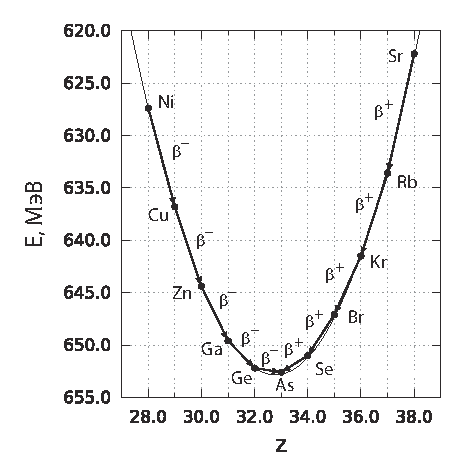
\includegraphics[width=.38\textwidth]{75}}
            \\ \cline{1-6}
            % -----------------------------------------
            Никель & Ni & 28 & 627,4 & Бета\( ^- \) &
            \( \el{Ni}{75}{28}\, \to\ \el{Cu}{75}{29} + e^- + \tilde{\nu} \) &
            \\ \cline{1-5}
            Медь & Cu & 29 & 636,8 & Бета\( ^- \) &
            \( \el{Cu}{75}{29}\, \to\ \el{Zn}{75}{30} + e^- + \tilde{\nu} \) &
            \\ \cline{1-5}
            Цинк & Zn & 30 & 644,4 & Бета\( ^- \) &
            \( \el{Zn}{75}{30}\, \to\ \el{Ga}{75}{31} + e^- + \tilde{\nu} \) &
            \\ \cline{1-5}
            Галлий & Ga & 31 & 649,6 & Бета\( ^- \) &
            \( \el{Ga}{75}{31}\, \to\ \el{Ge}{75}{32} + e^- + \tilde{\nu} \) &
            \\ \cline{1-5}
            Германий & Ge & 32 & 652,2 & Бета\( ^- \) &
            \multirow{2}{*}{\( \el{Ge}{75}{32}\, \to\ \el{As}{75}{33} + e^-
            + \tilde{\nu} \)} & \\ \cline{1-5}
            Мышьяк & As & 33 & 652,6 & Стабильный изобар &
            \multirow{3}{*}{\( \el{Se}{75}{34} \to\ \el{As}{75}{34} + e^+
            + \nu \)} & \\ \cline{1-5}
            Селен & Se & 34 & 651,0 & Бета\( ^+ \) & & \\ \cline{1-5}
            Бром & Br & 35 & 647,1 & Бета\( ^+ \) &
            \( \el{Br}{75}{35} \to\ \el{Se}{75}{34} + e^+ + \nu \) &
            \\ \cline{1-5}
            Криптон & Kr & 36 & 641,5 & Бета\( ^+ \) &
            \( \el{Kr}{75}{36} \to\ \el{Br}{75}{35} + e^+ + \nu \) &
            \\ \cline{1-5}
            Рубидий & Rb & 37 & 633,6 & Бета\( ^+ \) &
            \( \el{Rb}{75}{37} \to\ \el{Kr}{75}{36} + e^+ + \nu \) &
            \\ \cline{1-5}
            Стронций & Sr & 38 & 622,2 & Бета\( ^+ \) &
            \( \el{Sr}{75}{38} \to\ \el{Rb}{75}{37} + e^+ + \nu \) &
            \\ \cline{1-6}
        \end{tabular}
    \end{table}

    Энергия связи элемента \( \el{As}{75}{33} \): \( E_\emph{св} = 655,7 \)~МэВ.

    \pagebreak

    \begin{table}[h!]
        \center
        \caption{\( A = 109 \)}
        \begin{tabular}{|C{.08}|C{.065}|C{.02}|C{.05}|C{.1}||C{.2}|C{.38}} \cline{1-6}
            Название & Элемент & \( Z \) & \( E_\emph{св} \), МэВ & Распад &
            Формула распада &
            \multirow{15}{*}{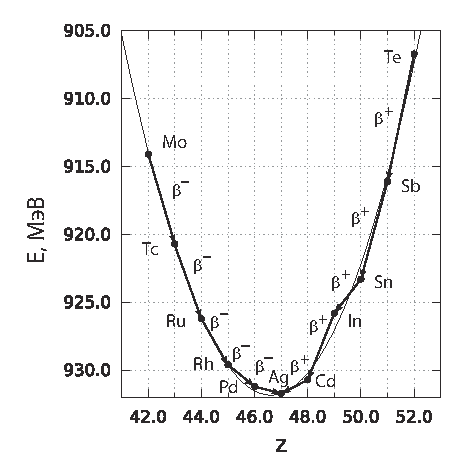
\includegraphics[width=.38\textwidth]{109}}
            \\ \cline{1-6}
            % -----------------------------------------
            Молибден & Mo & 42 & 914,1 & Бета\( ^- \) &
            \( \el{Mo}{109}{42}\, \to\ \el{Tc}{109}{43} + e^- + \tilde{\nu} \) &
            \\ \cline{1-5}
            Технеций & Tc & 43 & 920,7 & Бета\( ^- \) &
            \( \el{Tc}{109}{43}\, \to\ \el{Ru}{109}{44} + e^- + \tilde{\nu} \) &
            \\ \cline{1-5}
            Рутений & Ru & 44 & 926,2 & Бета\( ^- \) &
            \( \el{Ru}{109}{44}\, \to\ \el{Rh}{109}{45} + e^- + \tilde{\nu} \) &
            \\ \cline{1-5}
            Родий & Rh & 45 & 929,6 & Бета\( ^- \) &
            \( \el{Rh}{109}{45}\, \to\ \el{Pd}{109}{46} + e^- + \tilde{\nu} \) &
            \\ \cline{1-5}
            Палладий & Pd & 46 & 931,2 & Бета\( ^- \) &
            \multirow{2}{*}{\( \el{Pd}{109}{46}\, \to\ \el{Ag}{109}{47} + e^-
            + \tilde{\nu} \)} & \\ \cline{1-5}
            Серебро & Ag & 47 & 931,7 & Стабильный изобар &
            \multirow{3}{*}{\( \el{Cd}{109}{48} \to\ \el{Ag}{109}{47} + e^+
            + \nu \)} & \\ \cline{1-5}
            Кадмий & Cd & 48 & 930,7 & Бета\( ^+ \) & & \\ \cline{1-5}
            Индий & In & 49 & 925,8 & Бета\( ^+ \) &
            \( \el{In}{109}{49} \to\ \el{Cd}{109}{48} + e^+ + \nu \) &
            \\ \cline{1-5}
            Олово & Sn & 50 & 923,3 & Бета\( ^+ \) &
            \( \el{Sn}{109}{50} \to\ \el{In}{109}{49} + e^+ + \nu \) &
            \\ \cline{1-5}
            Сурьма & Sb & 51 & 916,1 & Бета\( ^+ \) &
            \( \el{Sb}{109}{51} \to\ \el{Sn}{109}{50} + e^+ + \nu \) &
            \\ \cline{1-5}
            Теллур & Te & 52 & 906,7 & Бета\( ^+ \) &
            \( \el{Te}{109}{52} \to\ \el{Sb}{109}{51} + e^+ + \nu \) &
            \\ \cline{1-6}
        \end{tabular}
    \end{table}

    Энергия связи элемента \( \el{Ag}{109}{47} \): \( E_\emph{св} = 933,3 \)~МэВ.

    \begin{table}[h!]
        \center
        \caption{\( A = 139 \)}
        \begin{tabular}{|C{.08}|C{.065}|C{.02}|C{.05}|C{.1}||C{.2}|C{.38}} \cline{1-6}
            Название & Элемент & \( Z \) & \( E_\emph{св} \), МэВ & Распад &
            Формула распада &
            \multirow{15}{*}{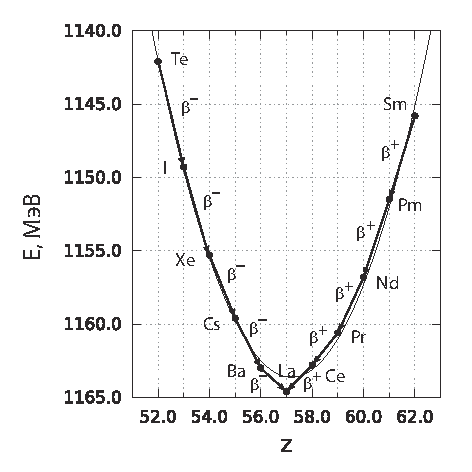
\includegraphics[width=.38\textwidth]{139}}
            \\ \cline{1-6}
            % -----------------------------------------
            Теллур & Te & 52 & 1142,1 & Бета\( ^- \) &
            \( \el{Te}{139}{52}\, \to\ \el{I}{139}{53} + e^- + \tilde{\nu} \) &
            \\ \cline{1-5}
            Йод & I & 53 & 1149,3 & Бета\( ^- \) &
            \( \el{I}{139}{53}\, \to\ \el{Xe}{139}{54} + e^- + \tilde{\nu} \) &
            \\ \cline{1-5}
            Ксенон & Xe & 54 & 1155,3 & Бета\( ^- \) &
            \( \el{Xe}{139}{54}\, \to\ \el{Cs}{139}{55} + e^- + \tilde{\nu} \) &
            \\ \cline{1-5}
            Цезий & Cs & 55 & 1159,6 & Бета\( ^- \) &
            \( \el{Cs}{139}{55}\, \to\ \el{Ba}{139}{56} + e^- + \tilde{\nu} \) &
            \\ \cline{1-5}
            Барий & Ba & 56 & 1163,0 & Бета\( ^- \) &
            \multirow{2}{*}{\( \el{Ba}{139}{56}\, \to\ \el{La}{139}{57} + e^-
            + \tilde{\nu} \)} & \\ \cline{1-5}
            Лантан & La & 57 & 1164,6 & Стабильный изобар &
            \multirow{3}{*}{\( \el{Ce}{139}{58} \to\ \el{La}{139}{57} + e^+
            + \nu \)} & \\ \cline{1-5}
            Церий & Ce & 58 & 1162,8 & Бета\( ^+ \) & & \\ \cline{1-5}
            Празеодим & Pr & 59 & 1160,6 & Бета\( ^+ \) &
            \( \el{Pr}{139}{59} \to\ \el{Ce}{139}{58} + e^+ + \nu \) &
            \\ \cline{1-5}
            Неодим & Nd & 60 & 1156,8 & Бета\( ^+ \) &
            \( \el{Nd}{139}{60} \to\ \el{Pr}{139}{59} + e^+ + \nu \) &
            \\ \cline{1-5}
            Прометий & Pm & 61 & 1151,5 & Бета\( ^+ \) &
            \( \el{Pm}{139}{61} \to\ \el{Nd}{139}{60} + e^+ + \nu \) &
            \\ \cline{1-5}
            Самарий & Sm & 62 & 1145,8 & Бета\( ^+ \) &
            \( \el{Sm}{139}{62} \to\ \el{Pm}{139}{61} + e^+ + \nu \) &
            \\ \cline{1-6}
        \end{tabular}
    \end{table}

    Энергия связи элемента \( \el{La}{139}{57} \): \( E_\emph{св} = 1159,7 \)~МэВ.

    \vspace*{2em}

    \emph{Вывод:} был проведён опыт, по результатам которого были построены
    семейства парабол, иллюстрирующих \( \beta \)-превращения для чётных и
    нечётных значений массового числа \( A \), и вычислены значения энергий
    связи различных элементов.
\end{document}
